\chapter{Podstawy teoretyczne}

Niniejszy rozdział podsumowuje stan wiedzy na temat technologii wykorzystywanych przy konstrukcji tablicy. Omawia takie zagadnienia jak wyświetlacze matrycowe LED i~sposób ich sterowania, interfejs komunikacyjny USB i~karty pamięci typu SD.~Zamieszczono również podstawowe informacje na temat typografii z~racji wykorzystywania w~projekcie samodzielnie tworzonych fontów. Dołączono również spis używanych narzędzi programistycznych.

\section{Wyświetlacz matrycowy LED i~sterowanie multipleksowe}

\textit{Light-emitting diode}, dioda elektroluminescencyjna jest półprzewodnikowym elementem elektronicznym emitującym światło na skutek przepływającego przez nią prądu. Pod względem elektrycznym element ten zachowuje się jak zwykła dioda, pozwalając na przepływ prądu tylko, gdy jest on zgodny z~kierunkiem przewodzenia diody oraz gdy spadek napięcia na niej przekracza barierę potencjału złącza p-n, której wartość zależy od rodzaju zastosowanego półprzewodnika. 

Zasadniczym elementem tablicy świetlnej są wyświetlacze LED typu \mbox{JZM23882ASR} o~wymiarach zewnętrznych $53 \times 53$ mm, posiadające 64 diody LED koloru czerwonego zorganizowane w~matrycę o~wymiarach $8 \times 8$. Natężenie prądu przepływającego przez diodę może sięgać $30$ mA; w~projekcie, kierując się kompromisem między jasnością i~niezawodnością, ustalono prąd na $18$ mA.

\begin{figure}[t]
    \begin{center}
       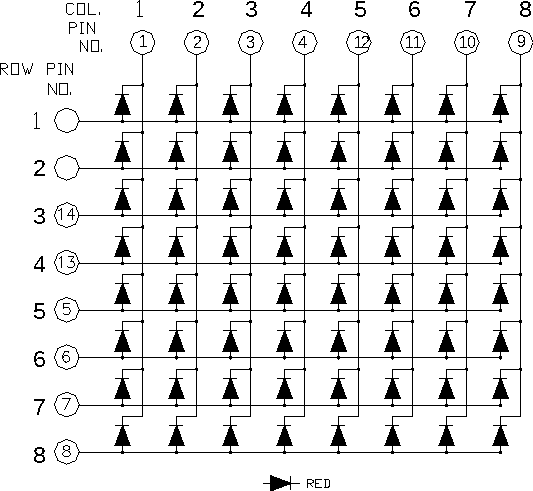
\includegraphics[width=0.8\textwidth]{figures/ledmatrix.pdf}
    \end{center}

    \caption{Schemat ideowy wyświetlacza matrycowego LED typu \mbox{JZM23882ASR-GW}. Źródło \cite{ds-wysw}.}
    \label{schemat-wysw}
\end{figure}

Sterowanie każdą komórką wyświetlacza niezależnie w~tradycyjny sposób wymagałoby $ 8 \times 8 + 1 = 65 $ wyprowadzeń (64 katody i~jedna wspólna anoda). By ilość tą zmniejszyć, producent zastosował odmienny sposób sterowania: komórki umieszczone są w~węzłach siatki utworzonej z~przecinających się linii anod i~katod, co pokazane jest na rysunku \ref{schemat-wysw}.

Sterowanie multipleksowe wyświetlacza jest rodzajem sterowania dynamicznego, to znaczy, że w~celu uzyskania stabilnego obrazu należy z~odpowiednio dużą szybkością wysterowywać pojedynczą kolumnę lub wiersz, odczekać pewien czas a~następnie wysterowywać kolumnę lub wiersz następny. W~danej chwili aktywny jest tylko jeden wiersz/kolumna.

Wrażenie stabilnego obrazu powstaje dzięki bezwładności oka ludzkiego, które uśrednia szybko zmieniające się obrazy. Zakładając, że wyświetlacz ma osiem kolumn, obserwator odbiera wrażenie świecenia wiersza z~jedną ósmą swej maksymalnej jasności (zakładając liniowość percepcji oka). Praktyka pokazuje, że stabilny obraz uzyskuje się, gdy częstotliwość odświeżenia całego ekranu przekracza $250$ Hz \cite{sztuka2}.

W prezentowanym urządzeniu przełączanie aktywnej kolumny odbywa się co $200$ $\mu$s, co oznacza, że przerysowywanie ekranu odbywa się z~częstotliwością $312$ Hz.

\section{Mikrokontroler AVR typu AT90USB647}

\textit{AVR} to rodzina ośmiobitowych mikrokontrolerów jednoukładowych stworzona przez firmę Atmel. Została opracowana zgodnie z~założeniami zmodyfikowanej architektury harwardzkiej (rozdzielone pamięci danych i~programu, lecz wspólne szyny danych i~adresowa). W~pojedynczym układzie scalonym umieszczono, obok procesora, większość modułów niezbędnych do działania systemu mikroprocesorowego takich jak pamięć operacyjna, pamięć programu FLASH, timery systemowe, obwody wejścia/wyjścia itd. Fakt ten umożliwia budowanie urządzeń znacznie mniejszych i~pobierających mniej energii, niż porównywalne systemy złożone z~wielu układów scalonych.

Mikrokontroler jednoukładowy AT90USB647 jest przedstawicielem rodziny AVR, zastosowanym ze względu na zintegrowany sprzętowy interfejs USB strony urządzenia. Umożliwiło to łatwą implementację komunikacji tablicy świetlnej z~komputerem PC.~Poniżej omówiono pozostałe właściwości i~moduły mikrokontrolera, które wykorzystywane były w~konstrukcji tablicy, opracowane na podstawie noty katalogowej \cite{ds-avr}. Schemat blokowy przedstawiono na rysunku \ref{blokowy-avr}.

\begin{figure}[t]
    \begin{center}
       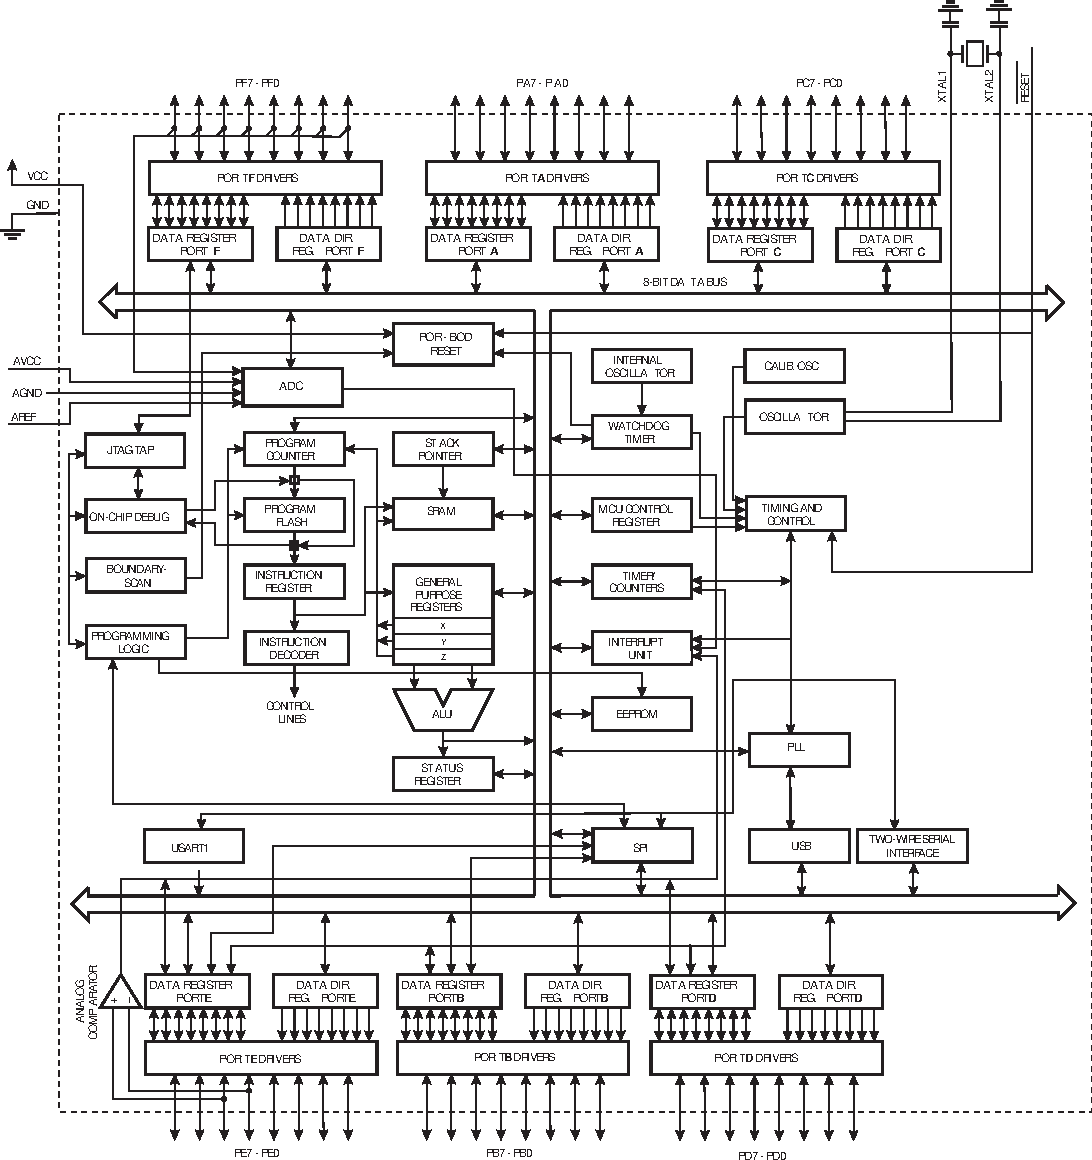
\includegraphics[width=\textwidth]{figures/avrdiagram.pdf}
    \end{center}

    \caption{Schemat blokowy mikrokontrolera AT90USB647. Źródło: \cite{ds-avr}.}
    \label{blokowy-avr}
\end{figure}

\begin{itemize}

\item Architektura typu RISC: 135 instrukcji, z~czego większość wykonywana w~jednym cyklu zegara, 32 rejestry ogólnego przeznaczenia, zegar do $16$ MHz,

\item $64$ kB pamięci FLASH przeznaczonej na kod wykonywalny,

\item $4$ kB pamięci operacyjnej RAM,

\item interfejs diagnostyczny JTAG (niewykorzystywany),

\item wbudowany interfejs USB 2.0 \textit{full-speed} i~\textit{low-speed} typu \textit{device} lub \textit{On-The-Go}, wykorzystywany tryb urządzenia i~transfery masowe dla klasy \textit{Mass Storage},

\item dwa przerwania zewnętrzne, dwa przerwania reagujące na zbocze konfigurowalne na wielu wyprowadzeniach,

\item dwa zegary/liczniki 16-bitowe pozwalające na zliczanie impulsów z~zegara taktującego lub zewnętrznego źródła z~zastosowaniem lub nie dzielnika częstotliwości, generujące przerwania przy przepełnieniu lub osiągnięciu wartości przechowywanej w~rejestrach porównujących. Wykorzystywane do generowania przerwań obsługujących wyświetlacz matrycowy, gwarantujące odświeżanie w~deterministycznym czasie,

\item licznik czasu rzeczywistego (RTC) z~zewnętrznym oscylatorem niezależnym od zegara głównego, niezbędny do implementacji zegara czasu urzędowego z~kalendarzem, generujący przerwania co sekundę, również w~trybach obniżonego poboru mocy,

\item interfejs SPI wspierający tryb \textit{master} i~\textit{slave} --- używany do komunikacji z~kartą SD oraz szeregowego programowania mikrokontrolera przez złącze ISP,

\item pozostałe, niewykorzystywane podsystemy (większość z~nich może generować przerwania): sześć kanałów PWM, komparator analogowy, interfejs $I^{2}C$, uniwersalny interfejs szeregowy (min.~RS232C), 10-bitowy przetwornik analogowo-cyfrowy, dwa timery/liczniki ośmiobitowe,

\item obwody odpowiadające za reset mikrokontrolera i~kontrolę napięcia zasilania (\mbox{\textit{Brown-Out}}),

\item \textit{watchdog} --- podsystem resetujący mikrokontroler w~przypadku, gdy mikrokontroler wpadnie w~martwą pętlę, co skutkuje zawieszeniem wykonywania się programu, 

\item wewnętrzny oscylator RC i~oscylator kwarcowy,

\item tryby obniżonego poboru mocy: \textit{Idle, ADC Noise Reduction, \mbox{Power-save}, \mbox{Power-down}, Standby} i~\textit{Extended Standby}.

\end{itemize}


\section{Magistrala USB i~klasa pamięci masowej}

USB (ang. \textit{Universal Serial Bus}) to standard definiujący warstwę fizyczną i~programową interfejsu łączącego różne urządzenia peryferyjne z~komputerem PC. W~chwili pisania niniejszej pracy aktualną jest wersja standardu 3.0. Dokument ten definiuje sposoby połączeń, kształty gniazd i~wtyków, sposoby implementacji modułów po stronie hosta (komputer PC) i~samych urządzeń oraz reprezentację ich w~systemach operacyjnych.

Magistrala USB ma topologię drzewa. Wszystkie urządzenia połączone są z~\textit{hostem} przy pomocy \textit{hubów}. Na samym szczycie znajduje się hub główny. Możliwe jest podłączenie do 127 urządzeń.~Szybkość przesyłu danych może wynosić od 1.5, 12, 480 MBit/s lub 5 GBit/s dla standardu 3.0. Urządzenia posiadają od jednego do kilku tzw. punktów końcowych (ang.  \textit{endpoint}). Między punktami końcowymi urządzenia i~hosta może być zestawiony wirtualny kanał komunikacyjny, w~którym płyną dane do i~z~urządzenia. Fizycznie przewód USB ma cztery linie: masę, zasilanie $+5$ V $500$ mA i~sygnałowe: D+, D-. Linie sygnałowe pracują różnicowo przy poziomach logicznych 0~V i~3,3~V.

Mając na uwadze uniwersalność magistrali standard definiuje cztery rodzaje połączeń (transferów) między punktami końcowymi: kontrolny, przerwaniowy, masowy i~izochroniczny. Każde urządzenie musi udostępniać co najmniej jeden kontrolny punkt końcowy. Transfer ten charakteryzuje się małą ilością danych w~ramce i~kontrolą poprawności. Jak wskazuje nazwa, służy on do kontroli pracy urządzenia i~ustalania jego konfiguracji. Transfer przerwaniowy posiada podobną charakterystykę do kontrolnego. Służy on do przesyłania małych porcji danych w~gwarantowanym czasie. Klasycznym zastosowaniem jest myszka komputerowa, gdzie przekazywanie bieżącej pozycji jest szczególnie istotne dla komfortu użytkownika (szczególnie w~grach).

Transfery masowy i~izochroniczny służą do przesyłu dużych ilości danych. Transfer izochroniczny wymusza dodatkowo natychmiastowość ich dostarczenia kosztem kontroli poprawności. Źle dostarczone są bezpowrotnie tracone. Istotne jest to w~zastosowaniach audio. Pojedyncze przekłamanie jest z~reguły praktycznie niesłyszalne, natomiast konieczność ponownego transferu pakietu danych spowodowałaby chwilową przerwę w~odtwarzaniu dźwięku. Dla transferu masowego priorytetem jest poprawność. Używają go wszystkie urządzenia pamięci masowej: \textit{pendrive}, dyski itd. Opisywana tablica korzysta głównie z~transferów masowych, z~racji wykorzystywanej klasy urządzenia \textit{Mass Storage}.

By przyporządkować podobne urządzenia wielu producentów do jednej grupy standard definiuje wiele \textit{klas}. Najważniejsze z~nich to: drukarka, pamięć masowa, hub, urządzenie komunikacji z~użytkownikiem (ang. \textit{Human Interface Device}), do której należą na przykład myszki i~klawiatury. Oprócz klasy, każde urządzenie posiada parę dwóch liczb identyfikatora producenta (\textit{Vendor ID}) i~produktu (\textit{Product ID}). Kod producenta przydzielany jest przez organizację \textit{usb.org}, twórców standardu.

\textbf{Klasa pamięci masowej} została zastosowana do implementacji komunikacji tablicy z~komputerem PC, dzięki czemu obecna w~urządzeniu karta SD widoczna jest w~systemie operacyjnym jako dysk twardy, niewymagający dodatkowych sterowników. Rozwiązanie takie podyktowane zostało prostotą obsługi przez użytkownika oraz istnieniem gotowych bibliotek implementujących wyżej wymienioną funkcjonalność, będących częścią pakietu \textit{LUFA}.

Protokół komunikacji w~omawianej klasie nie jest zależny od systemu plików i~działa na jednostkach danych --- blokach, których rozmiar jest charakterystyczny dla urządzenia, lecz zwykle wynosi 64 bajty. Na komunikację składają się trzy fazy \cite{interfejsy}:

\begin{enumerate}
\item wysłanie do urządzenia rozkazu,
\item odebranie statusu wykonania rozkazu,
\item odebranie danych, jeżeli zażądano odczytu.
\end{enumerate}

Pojedyncze urządzenie pamięci masowej może definiować wiele logicznych urządzeń LUN (ang. \textit{Logical UNit}), do których kierowane są polecenia. Bloki poleceń zawierają rozkazy zgodne z~tradycyjnymi interfejsami, jak ATA/ATAPI lub SCSI, co upraszcza implementację zarówno po stronie urządzenia, jak i~hosta. Oprócz nich stosowane są rozkazy dodatkowe, jak zerowanie urządzenia, przeładowanie buforów danych, sprawdzanie statusu itd.


\section{Karta SD}

\textit{Secure Digital} jest rodziną standardów przenośnych kart pamięci FLASH wywodzącą się z~wcześniejszego rozwiązania --- MMC, stosowaną w~wielu urządzeniach mobilnych, np. aparatach cyfrowych. Karta SD ma 9 wyprowadzeń i~wymiary $24 \times 32 \times 2.1$ mm. Na dzień pisania niniejszej pracy istnieją następujące wersje według pojemności:
\begin{itemize}
	\item SD --- pojemność do 4 GB,
	\item SDHC --- do 32 GB,
	\item SDXC --- do 2 TB pojemności
\end{itemize}
oraz rozmiaru:
\begin{itemize}
	\item Standard --- $ 24 \times 32 \times 2.1 $ mm,
	\item Mini --- $ 21.5 \times 20.0 \times 1.4 $ mm,
	\item Micro --- $ 15.0 \times 11.0 \times 1.0 $ mm.
\end{itemize}

Karta SD może komunikować się z~urządzeniem w~dwóch trybach: \textit{SD bus} oraz \textit{SPI bus}. SD bus jest własnościowym protokołem, co znaczy, że wymagana jest licencja na jego użycie. Tylko on pozwala na osiągnięcie pełnej szybkości transferu danych. Oprócz niego karty w~rozmiarze \textit{standard} implementują protokół zgodny z~interfejsem SPI, powszechnie stosowanym w~systemach wbudowanych. Karty w~rozmiarach \textit{mini} i~\textit{micro} mogą, lecz nie muszą być kompatybilne z~SPI.

Zasadniczym powodem zastosowania tego typu pamięci jest jej powszechność we wszelkiego typu urządzeniach przenośnych, jak aparaty cyfrowe, telefony komórkowe, nawigacje GPS itd. oraz łatwość komunikacji przez SPI z~mikrokontrolerem, który również wyposażony jest w~ten interfejs. Opis wyprowadzeń znajduje się na rysunku \ref{schemat-sd}. 

\begin{figure}[tb]
    \begin{center}
       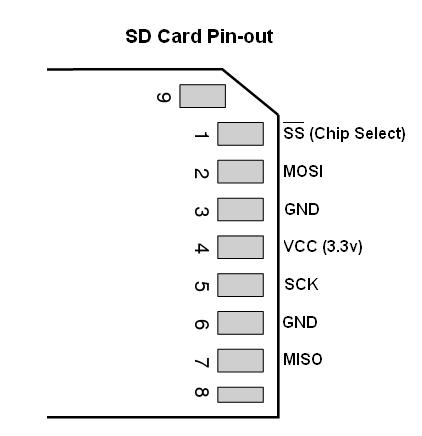
\includegraphics[width=0.4\textwidth]{figures/SD_pinout.jpg}
    \end{center}

    \caption{Opis wyprowadzeń karty SD w rozmiarze standard. Źródło \cite{sd1}.}
    \label{schemat-sd}
\end{figure}

Komunikacja z~kartą inicjowana jest zawsze przez urządzenie poprzez wysłanie \mbox{48-bitowego} rozkazu. Rozkaz składa się z~nagłówka, kodu operacji, argumentu oraz sumy kontrolnej. Urządzenie po przetworzeniu zapytania odpowiada \mbox{8-bitowym} statusem. Jeżeli zażądano odczytu, długość odpowiedzi to 40 bitów. Częstotliwość zegara taktującego (SCK) powinna mieścić się w granicach 100--400 kHz.

Do obsługi karty SD została użyta biblioteka \textit{sd\_raw}, która udostępnia podstawową funkcjonalność, jaką jest identyfikacja karty oraz odczyt i~zapis bloku pod wskazanym adresem. Jest to wystarczające do obsługi systemu plików FAT.

Dane na karcie przechowywane są w~postaci plików w~systemie FAT32. Do odczytu plików wykorzystano bibliotekę FatFS, którą połączono z~biblioteką sd\_raw zgodnie ze wskazówkami z~\cite{programowanie-avr}. Biblioteka ta umożliwia manipulację plikami w~sposób podobny to tego, jaki używany jest w~bibliotece standardowej języka C.

\section{Typografia i~fonty}

\textbf{Czcionką} nazywamy nośnik pojedynczego znaku drukarskiego. Wyróżniamy czcionki tradycyjne oraz komputerowe, gdzie znak drukarski zapisany jest w~postaci grafiki bitmapowej lub wektorowej \cite{fonts}. \textbf{Font}, nazywany potocznie czcionką, to zestaw znaków drukarskich o~wspólnych cechach \cite{fonts}.

Do najważniejszych cech czcionek należą styl, stopień, proporcjonalność i~szeryf. W~foncie proporcjonalnym poszczególne znaki różnią się szerokością, w~nieproporcjonalnej jest ona stała. Czcionki o~stałej szerokości zazwyczaj charakteryzują się niższą estetyką w~porównaniu z~proporcjonalnymi, ponieważ odległości między wąskimi znakami, jak np. ,,l'' są większe, niż między szerokimi, jak ,,W''.

\begin{figure}[t]
    \begin{center}
       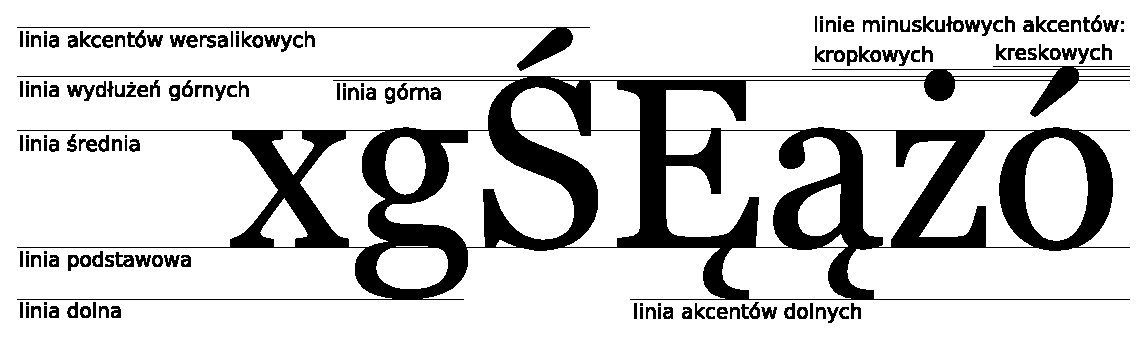
\includegraphics[width=0.8\textwidth]{figures/linie-pisma.pdf}
    \end{center}

    \caption{Linie pisma. Źródło: \url{pl.wikipedia.org/wiki/Plik:Linie-pisma.svg}.}

    \label{linie-pisma}
\end{figure}


Ważnym pojęciem dotyczącym czcionek są \textit{linie pisma}, które wyznaczają położenie liter w~pionie. Pokazuje to rysunek \ref{linie-pisma}. Jako że znaki mogą być niskie, wysokie, oraz mieć wydłużenia dolne, zostało zdefiniowane kilka takich linii \cite{fonts}.
\begin{itemize}
	\item \textbf{Linia podstawowa} pisma wyznacza dolną krawędź większości liter i~wszystkich cyfr, takich jak ,,a'', ,,B'', ,,c'',
	\item \textbf{linia dolna} znajduje się poniżej podstawowej, wskazuje dolną krawędź liter z~wydłużeniami dolnymi, takimi jak ,,g'', ,,j'', ,,y'',
	\item \textbf{linia średnia} pisma określa wysokość małych liter bez wydłużeń górnych, np. ,,a'', ,,e'', ,,m'',
	\item \textbf{linia górna} pisma określa górna krawędź wielkich liter, cyfr, i~małych liter z~wydłużeniami górnymi, jak ,,b'', ,,C'', ,,k'', ,,t''.
\end{itemize}

W urządzeniu zapisane są fonty bitmapowe w~trzech rozmiarach. Z~racji niskiej rozdzielczości matrycy i~ograniczonych zasobów sprzętowych ograniczono się do czcionek bezszeryfowych nieproporcjonalnych.

\section{Zastosowane narzędzia programistyczne}

W toku realizacji projektu posługiwano się wymienionymi niżej narzędziami programistycznymi. Wszystkie z~nich są darmowe do zastosowań niekomercyjnych, wiele z~nich ma licencję \textit{open source}. Wybór był najczęściej podyktowany ich popularnością oraz wcześniejszym doświadczeniem autorów w~ich używaniu.

\begin{itemize}
	\item Pakiet \textbf{avr-gcc} jest kompilatorem języka C/C++ dla mikrokontrolerów AVR.~Generuje on pliki binarne w~formacie \textit{Intel Hex} przeznaczone dla mikrokontrolera,
	\item \textbf{CadSoft EAGLE} do zaprojektowania schematu ideowego i~rysunku ścieżek płytki drukowanej sterownika. Umożliwia eksport do formatu Gerber, który jest powszechnie akceptowany przez wytwórnie płytek drukowanych,
	\item \textbf{IDE NetBeans} został wybrany ze względu na wygodny edytor formatek dla aplikacji okienkowych i~wieloplatformowość,
	\item \textbf{XVI32} jest popularnym edytorem szesnastkowym, był wykorzystywany przy testowaniu symulatora i~sterownika,
	\item rozproszony system kontroli wersji \textbf{git} umożliwił wydajną współpracę przy tworzeniu oprogramowania i~tekstu pracy.
\end{itemize}

